\adparagraph{Rating nDCG}
In Figure \ref{fig:andcg} we see the scores of the Rating nDCG measure. All methods generally have high levels of satisfaction according to the measure, with none scoring below 95 percent satisfaction.

Avg is ahead of the other methods, but it is also the only method using the average rating of all the candidate items for its recommendation. The remainder are mostly identical in performance to each other.
\begin{figure}[H]
	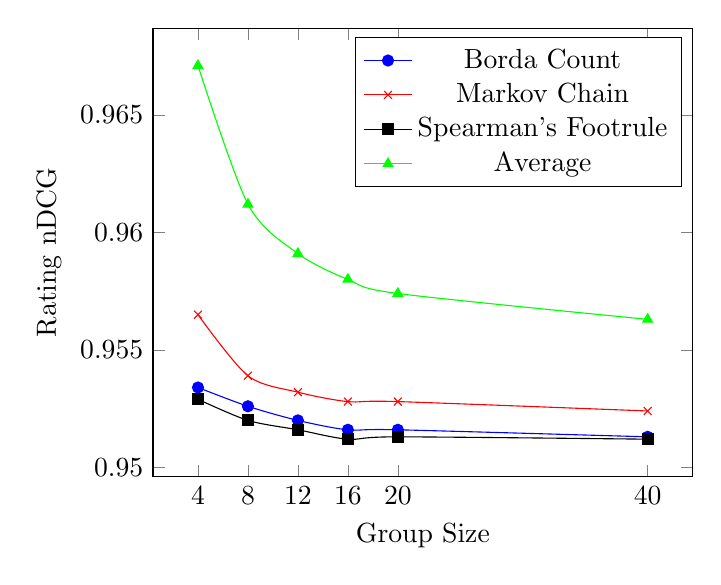
\begin{tikzpicture}
	\begin{axis}[
	y tick label style={
        /pgf/number format/.cd,
            precision=3,
        /tikz/.cd
    },
	xlabel=Group Size,
	ylabel=Rating nDCG,
	xtick = {4,8,12,16,20,40}]
	\addplot[smooth,mark=*,blue] plot coordinates {
		(4,0.9534)
		(8,0.9526)
		(12,0.952)
		(16,0.9516)
		(20,0.9516)
		(40,0.9513)
	};
	\addlegendentry{Borda Count}
	
	\addplot[smooth,color=red,mark=x] plot coordinates {
		(4,0.9565)
		(8,0.9539)
		(12,0.9532)
		(16,0.9528)
		(20,0.9528)
		(40,0.9524)
	};
	\addlegendentry{Markov Chain}
	
	\addplot[smooth,color=black,mark=square*] plot coordinates {
		(4,0.9529)
		(8,0.952)
		(12,0.9516)
		(16,0.9512)
		(20,0.9513)
		(40,0.9512)
	};
	\addlegendentry{Spearman's Footrule}
	
	\addplot[smooth,color=green,mark=triangle*] plot coordinates {
		(4,0.9671)
		(8,0.9612)
		(12,0.9591)
		(16,0.958)
		(20,0.9574)
		(40,0.9563)
	};
	\addlegendentry{Average}
	
	\end{axis}
	\end{tikzpicture}
	\caption{Results using Rating nDCG}\label{fig:andcg}
\end{figure}

As can be seen in Table \ref{tbl:andcg}, BC, \MC, and SF do not decrease in score from 16 to 20, and SF increases in score. In general, the fall in nDCG score is extremely low compared to the other measures. This could indicate, that the individual recommendations are biased towards some selection of items.

Among the remainder, while \MC does outperform both BC and SF, the difference is small.

\begin{table}[H]
	\centering
	\begin{tabular}{|l|lllll|}\hline
		& 4 to 8 & 8 to 12 & 12 to 16 & 16 to 20 & 20 to 40 \\\hline
		BC 	& 0.084	& 0.063	& 0.42	& 0		& 0.032 \\
		MC  & 0.27	& 0.73	& 0.42	& 0		& 0.042 \\
		SF  & 0.094	& 0.042	& 0.042	&-0.011	& 0.011 \\
		Avg	& 0.61	& 0.22 	& 0.11	& 0.063	& 0.11  \\ \hline
	\end{tabular}
	\caption{Percentage decrease between the groups for Rating nDCG}
	\label{tbl:andcg}
\end{table}

Table \ref{tbl:andcg_ttest} shows the t-test results for Rating nDCG. For BC and SF, there are two cases, which has been marked in bold, where the difference is not significant enough to not be considered random. It can also be seen that the p-values for all but Avg are many orders of magnitudes smaller than seen for other measures, due to the similarity in the results.

\begin{table}[H]
	\centering
	\begin{tabular}{|l|llllll|}\hline
		& 4 & 8 & 12 & 16 & 20 & 40 \\\hline
		BC/MC	& $5e^{-64}$	& $5e^{-38}$	& $2e^{-37}$	& $3e^{-58}$	& $3e^{-60}$ & $5e^{-70}$ \\
		BC/SF	& \textbf{0.058}	& $1e^{-5}$	& $1e^{-5}$	& $2e^{-4}$	& $5e^{-5}$ & \textbf{0.089} \\
		BC/Avg	& $1e^{-251}$	& $2e^{-275}$ 	& $5e^{-299}$	& 0	& 0 & 0 \\
		MC/SF	& $1e^{-49}$	& $3e^{-52}$ 	& $2e^{-55}$	& $7e^{-62}$	& $6e^{-66}$ & $8e^{-68}$ \\
		MC/Avg	& $9e^{-221}$	& $7e^{-247}$ 	& $1e^{-266}$	& $3e^{-296}$	& $2e^{-308}$ & 0 \\
		SF/Avg	& $5e^{-212}$	& $1e^{-262}$ 	& $6e^{-280}$	& $3e^{-287}$	& $4e^{-305}$ & 0 \\ \hline
	\end{tabular}
	\caption{P-values for Rating nDCG t-test}
	\label{tbl:andcg_ttest}
\end{table}